\documentclass[compress]{beamer}
\usepackage[utf8x]{inputenc}
\usepackage{default}
\usepackage{graphics}
\useinnertheme{rounded}
\usecolortheme{whale}
\useoutertheme[subsection=false]{miniframes}
\graphicspath{{figures/}}

\setbeamertemplate{footline}[frame number]
\beamertemplatenavigationsymbolsempty

\title{Novelty Detection for Visual Place Classification}
\author{André Susano Pinto\inst{1}}
\date{February 1, 2011}

\institute[FEUP] {
 \inst{1}Faculdade de Engenharia da Universidade do Porto
}

\begin{document}

\AtBeginSection[]{\begin{frame}\frametitle{Outline}\tableofcontents[currentsection]\end{frame}}

\begin{frame}
 \titlepage

    Supervisors:
    \begin{itemize}
    \item Luis Paulo Reis
    \item Andrzej Pronobis
    \end{itemize}
\end{frame}

\begin{frame}{Outline}
 \tableofcontents
\end{frame}

\section{Problem Definition and Motivation}
\subsection{Place Classification}
\begin{frame}{Place Classification}
\begin{figure}
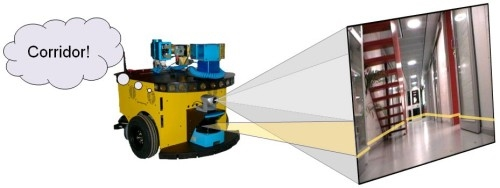
\includegraphics[width=0.75\textwidth]{place_classification}
\end{figure}
Mapping of robot location to concepts:
\begin{itemize}
\item Improves human interaction.
\item High-level and robust localization information.
\item Knowledge about room categories and their properties.
\item Context-aware decisions\cite{dey2000towards}.
\end{itemize}
\end{frame}

\subsection{Novelty Detection}
\begin{frame}{Novelty Detection}
\begin{figure}
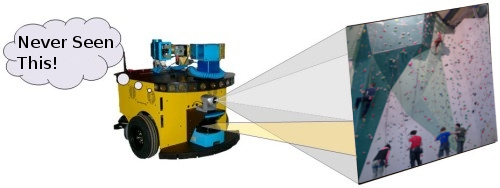
\includegraphics[width=0.75\textwidth]{novelty_detection}
\end{figure}

\begin{quotation}
Novelty detection is the identification of new or unknown data or signal that a machine learning system is not aware of during training\cite{markou2003novelty}.
\end{quotation}
\begin{itemize}
\item Operate in unknown environs.
\item Model of what is known.
\item Self-extend knowledge.
\end{itemize}
\end{frame}

\subsection{Goals}
\begin{frame}{Goals}


\begin{itemize}
\item Evaluation of a property-based semantic mapping system for mobile robots on a real world visual database\cite{pronobis2011exploiting}.
\vfill
\item Applying state-of-the-art novelty detection machine learning algorithms to the problem of visual place categorization.
\end{itemize}
\end{frame}



%%%%%%%%%%%%%%%%%%%%%%%%%%%%%%%%%%%%%%%%%%%%%%%%%%%%%%%%%%%%%%%%%
%%%%%%%%%%%%%%%%%%%%%%%%%%%%%%%%%%%%%%%%%%%%%%%%%%%%%%%%%%%%%%%%%
\section{Background and State-of-Art}

\subsection{Classification}

\begin{frame}{Classification}
\framesubtitle{Probability Estimation}

\begin{columns}[t]
    \column{.5\textwidth}
    \begin{figure}
        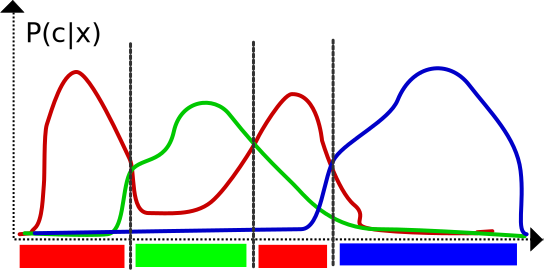
\includegraphics[width=.9\textwidth]{classification.pdf}
    \end{figure}
    \begin{quote}This is harder than the classification problem\cite{cortes1995support}\end{quote}.
    \column{.5\textwidth}
    Several approaches\cite{bishop2006pattern}:
    \begin{itemize}
        \item Nearest Neighbour
        \item Neural Networks
        \item Gaussian Mixture Models
        \item several others and extensions\dots 
    \end{itemize}
\end{columns}
\end{frame}

\begin{frame}{Classification}
\framesubtitle{Support Vector Machines}
    \begin{columns}[t]
    \column{.5\textwidth}
    \begin{figure}
        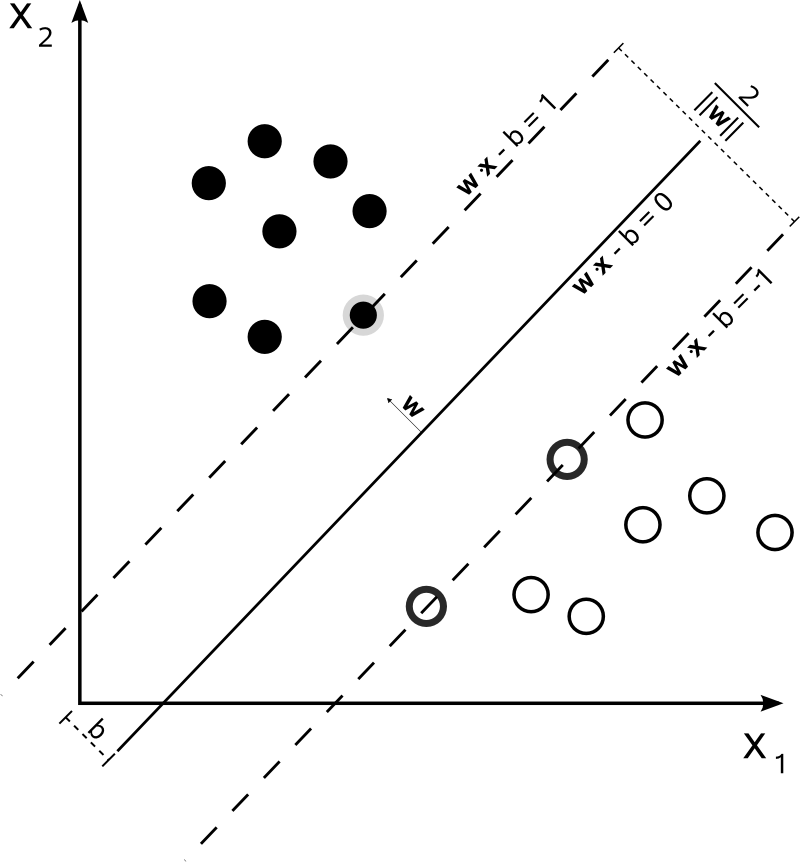
\includegraphics[width=.75\textwidth]{Svm_max_sep_hyperplane_with_margin}
    \end{figure}
        SVM uses a max-margin hyperplane to separate two classes.
    \column{.5\textwidth}
    \begin{block}{Kernel-Trick}
        Can be extended to non-linear classification:\\
        $K(x, y) = \phi(x)\cdot\phi(y)$
    \end{block}
    \begin{block}{Multi-class}
        Can be used in multi-class scenarios:
        \begin{itemize}
            \item One-Versus-One
            \item One-Versus-All
        \end{itemize}
    \end{block}
    \end{columns}
\end{frame}

%%%%%%%%%%%%%%%%%%%%%%%%%%%%%%%%%%%%%%%%%%%%%%%%%%
\subsection{Features}

\begin{frame}{Features}
\framesubtitle{Reasoning}
    \begin{itemize}
        \item Feature is a piece of information revealing useful information.
        \item Should be invariant and repeatable.
        \item Remove noise and useless information.
        \item Reduce the classification difficulty.
    \end{itemize}
\end{frame}


\begin{frame}{Features}
\framesubtitle{Visual Features - Local and Global}
    \begin{columns}[t]

    \column{.5\textwidth}
    \begin{figure}
        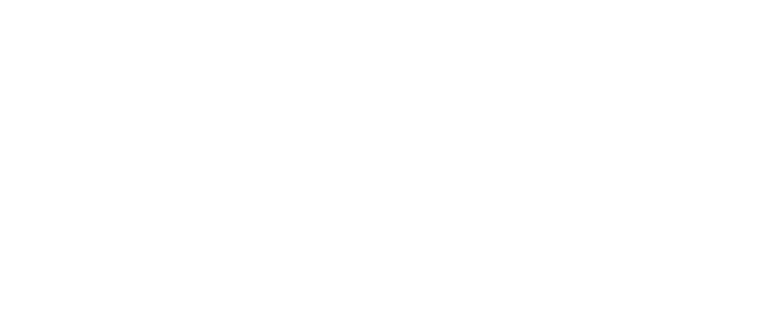
\includegraphics[width=\textwidth]{sift/sift}
        \caption{SIFT and other local features have been proven useful in object detection.}
    \end{figure}
    \column{.5\textwidth}
    \begin{figure}
    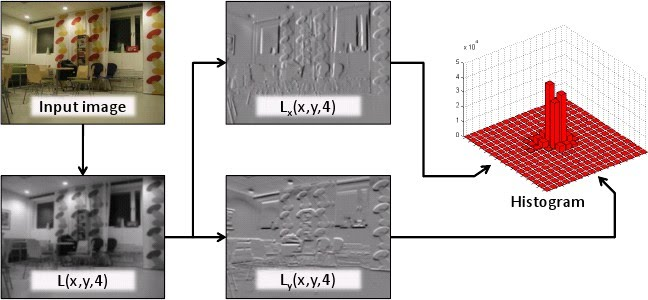
\includegraphics[width=\textwidth]{crfh_model}
    \caption{Composed Receptive Field Histograms can be used to extract appearance.}
    \end{figure}
    \end{columns}
\end{frame}

\begin{frame}{Features}
\framesubtitle{Others\dots}
    \begin{figure}
    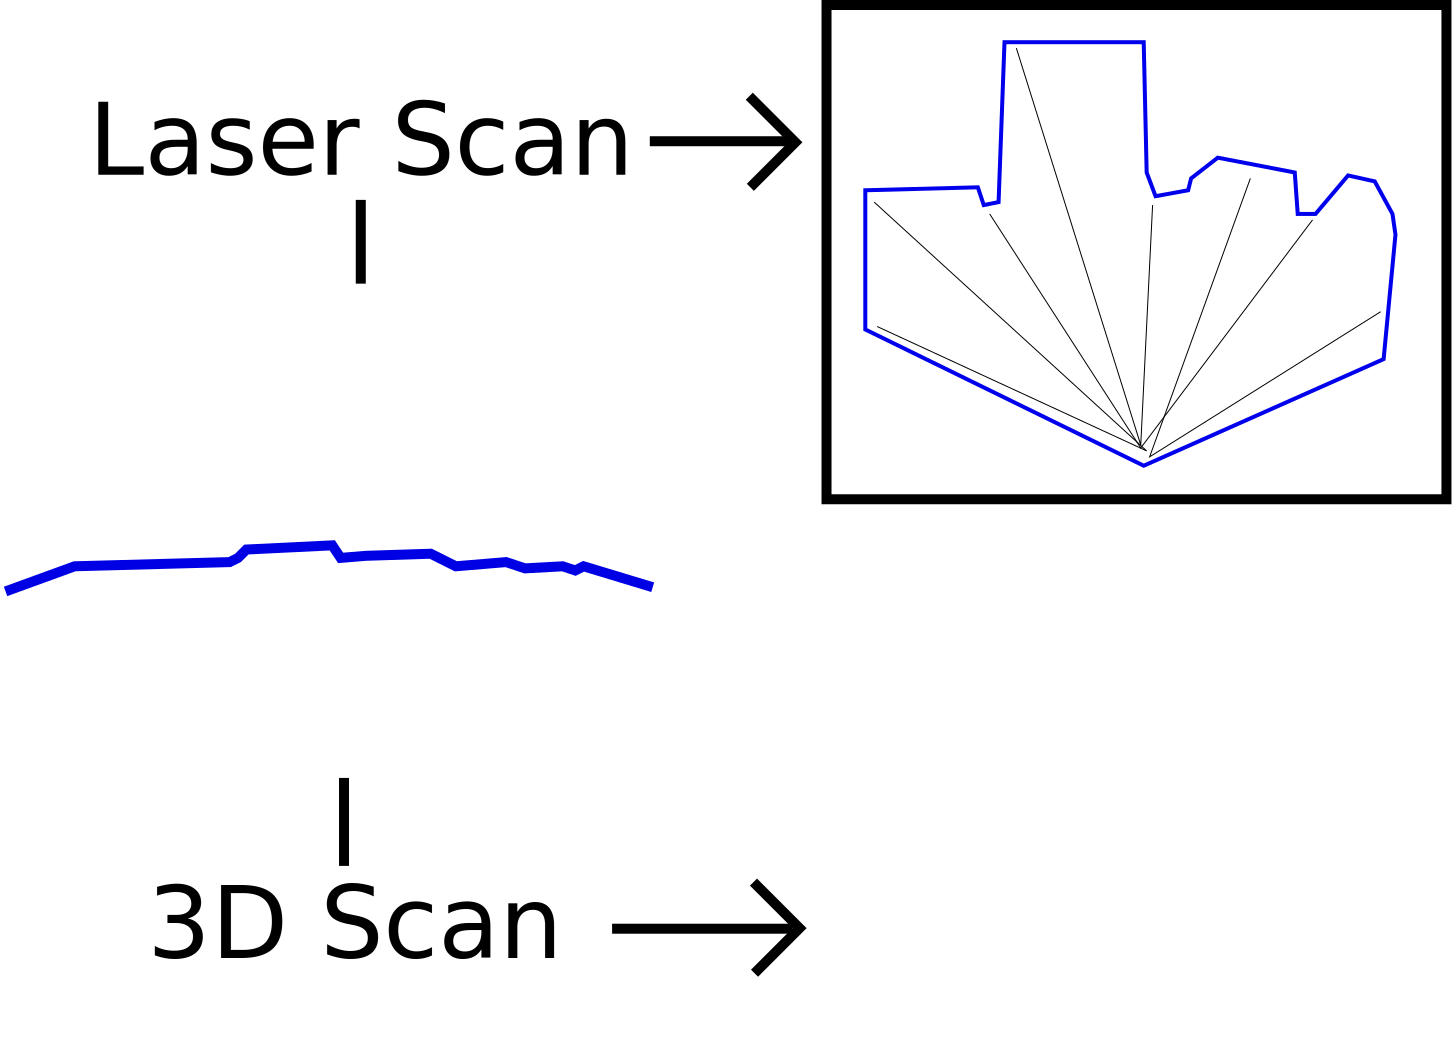
\includegraphics[width=0.60\textwidth]{laser_and_depth_input}
    \caption{Lasers can be used to extract useful features.}
    \end{figure}
\end{frame}

%%%%%%%%%%%%%%%%%%%%%%%%%%%%%%%%%%%%%%%%%%%%%%%%
\subsection{Novelty Detection}
\begin{frame}{Novelty Detection}
\framesubtitle{Probability}
    \begin{figure}
        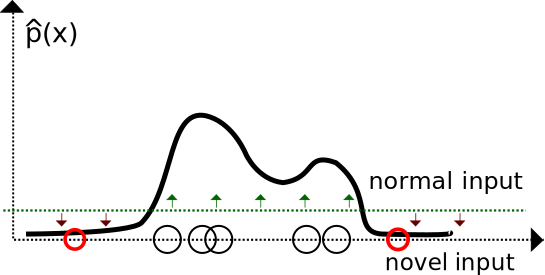
\includegraphics[width=0.75\textwidth]{novelty.pdf}
    \end{figure}
    Novelty detection can be modeled by calculating the probability of a given input being generated and triggering on that value\cite{bishop1994novelty}.
\end{frame}

\begin{frame}{Novelty Detection}
\framesubtitle{Kernel PCA}
    \begin{columns}[t]
    \column{.5\textwidth}
        \begin{itemize}
        \item Principal Component Analysis
        \item Extended for non-linear (kernel-trick)
        \item Radial Basis Function Kernel
        \item Use reconstruction error as novelty measure
        \item Good results on several applications
        \end{itemize}
    \column{.5\textwidth}
    \begin{figure}
        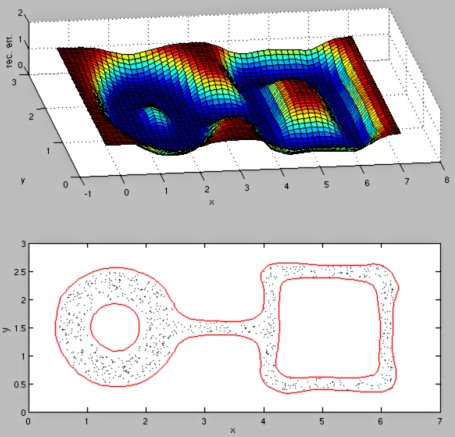
\includegraphics[width=0.9\textwidth]{ringlinesquare_kpca}
    \end{figure}
        Kernel PCA used on a strange shaped class\cite{Hoffmann2007863}.
    \end{columns}
\end{frame}

%%%%%%%%%%%%%%%%%%%%%%%%%%%%%%%%%%%%%%%%%%%%%%%%%
\subsection{Graphical Models}

\begin{frame}{Graphical Models}
    \begin{itemize}
        \item Represent a system of random variables
        \item Allow to model conditional independence
        \item Act as a filter of probability distributions
        \item Can calculate joint probabilities (inference).
    \end{itemize}
    \begin{columns}[t]
    \column{0.3\textwidth}
        \begin{figure}
            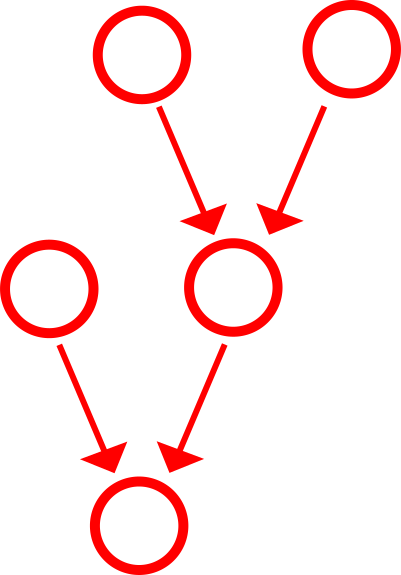
\includegraphics[width=0.5\textwidth]{graphical-models/BayesNet.pdf}
            \caption{Bayes Networks}
        \end{figure}
    \column{0.3\textwidth}
        \begin{figure}
            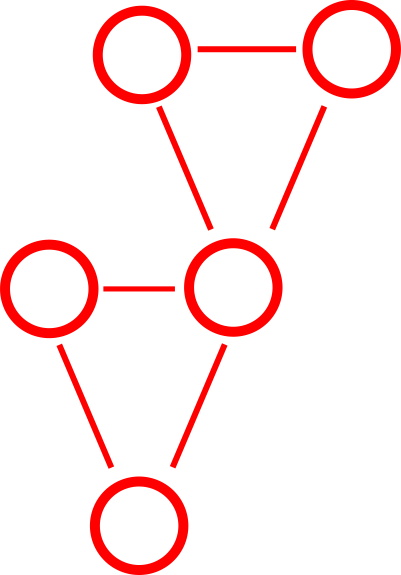
\includegraphics[width=0.5\textwidth]{graphical-models/MarkovRandomField}
            \caption{Markov Random Field}
        \end{figure}
    \column{0.3\textwidth}
        \begin{figure}
            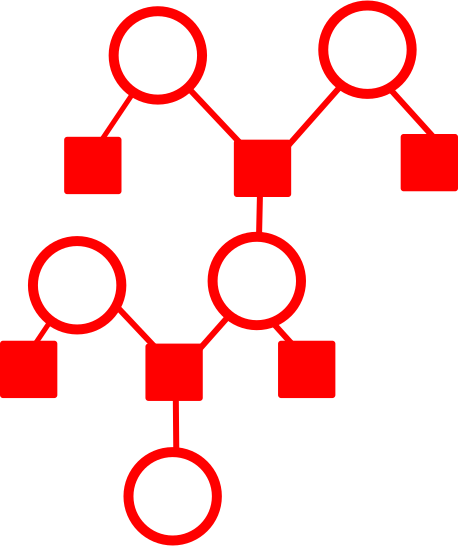
\includegraphics[width=0.60\textwidth]{graphical-models/FactorGraph.pdf}
            \caption{Factor Graph}
        \end{figure}
    \end{columns}
\end{frame}

\subsection{Related Work}
\begin{frame}{Related Work}
\begin{itemize}
    \item Object search studied for 20 years\cite{shubina2010}.
    \item Relation between object and room category\cite{galindo2005}.
    \item Bayes reasoning on top of deterministic presence of objects\cite{vasudevan2008}.
    \item Global and Local features for places indoor\cite{quattoni2009recognizing}.
\end{itemize}
\end{frame}

%%%%%%%%%%%%%%%%%%%%%%%%%%%%%%%%%%%%%%%%%%%%%%%%
%%%%%%%%%%%%%%%%%%%%%%%%%%%%%%%%%%%%%%%%%%%%%%%%
\section{Approach}
\subsection{Layers}
\begin{frame}{Layers}
    \begin{figure}
        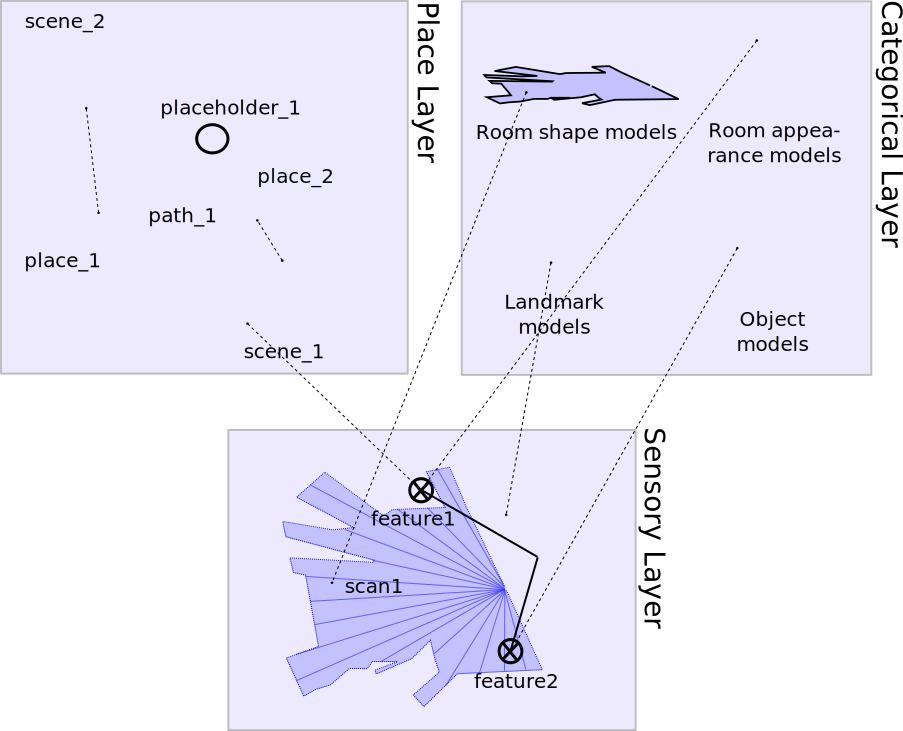
\includegraphics[width=0.65\textwidth]{system-representation/layers.pdf}
    \end{figure}
\end{frame}

\begin{frame}{Layers}
\framesubtitle{Conceptual Graph}
    \begin{figure}
        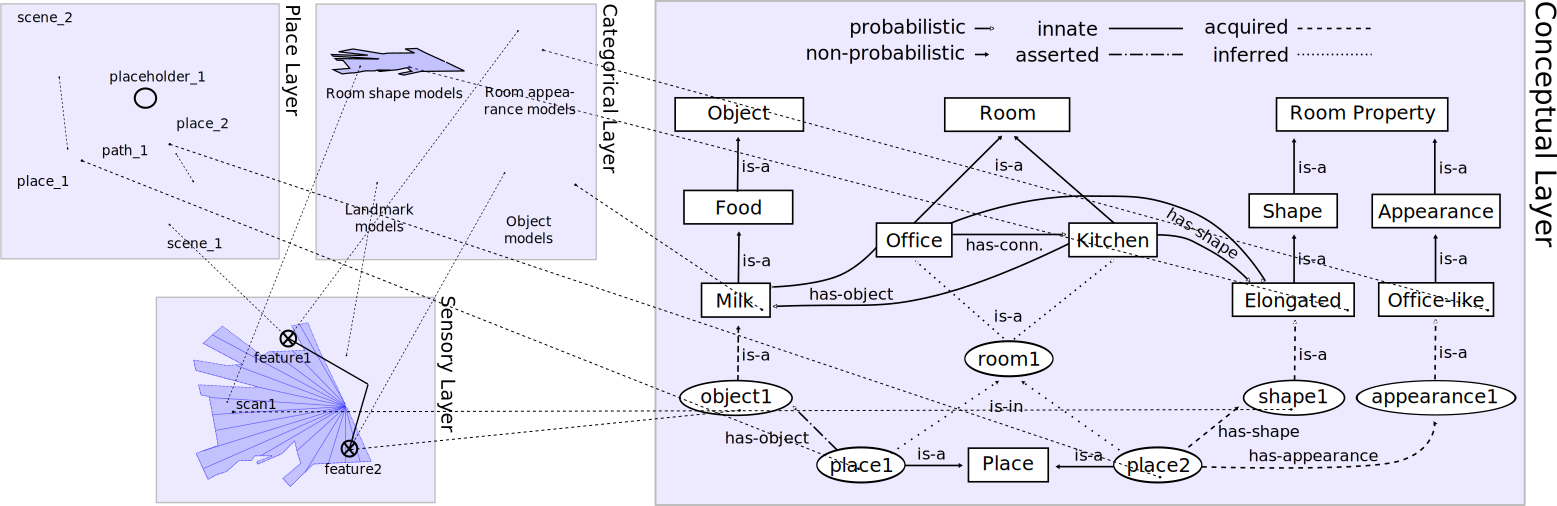
\includegraphics[width=\textwidth]{system-representation/graph.pdf}
    \end{figure}
\end{frame}

\begin{frame}{Layers}
\framesubtitle{Novelty Detection}
    \begin{figure}
        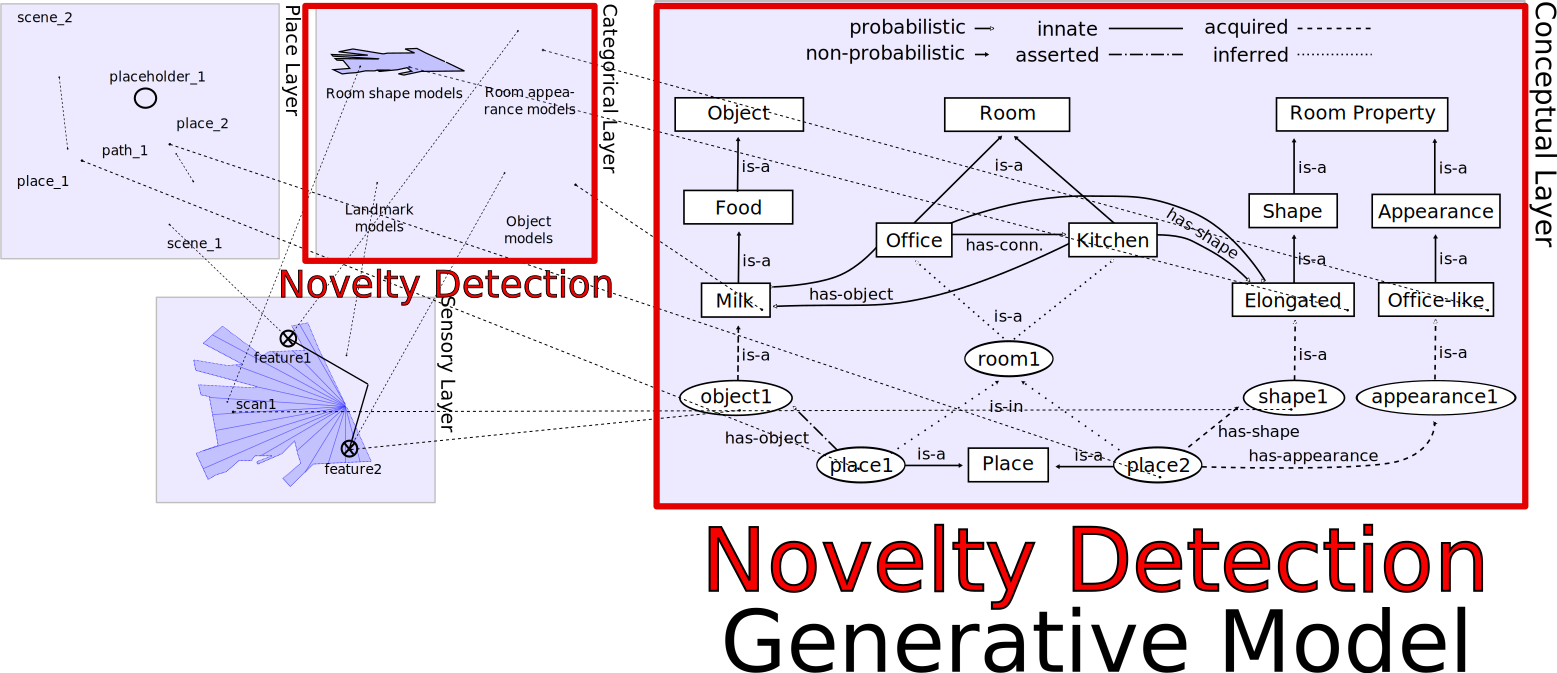
\includegraphics[width=\textwidth]{system-representation/novelty-detection.pdf}
    \end{figure}
\end{frame}

\subsection{Databases}
\begin{frame}{Databases}

\begin{figure}[!h]
\label{fig:cold-database-sample}
\begin{center}
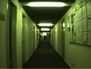
\includegraphics[width=0.15\textwidth]{cold/Saarbruecken_CR}
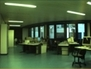
\includegraphics[width=0.15\textwidth]{cold/Saarbruecken_TR}
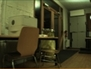
\includegraphics[width=0.15\textwidth]{cold/Freiburg_PA}
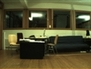
\includegraphics[width=0.15\textwidth]{cold/Freiburg_LO}
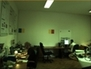
\includegraphics[width=0.15\textwidth]{cold/Ljubljana_LAB}
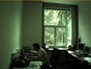
\includegraphics[width=0.15\textwidth]{cold/Ljubljana_2PO}

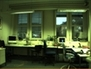
\includegraphics[width=0.15\textwidth]{cold/Saarbruecken_RL}
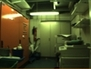
\includegraphics[width=0.15\textwidth]{cold/Saarbruecken_PA}
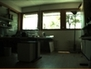
\includegraphics[width=0.15\textwidth]{cold/Freiburg_1PO}
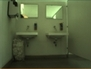
\includegraphics[width=0.15\textwidth]{cold/Freiburg_TL}
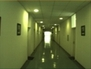
\includegraphics[width=0.15\textwidth]{cold/Ljubljana_CR}
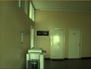
\includegraphics[width=0.15\textwidth]{cold/Ljubljana_PA}

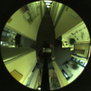
\includegraphics[width=0.15\textwidth]{cold/Saarbruecken_CR(1)}
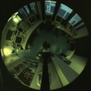
\includegraphics[width=0.15\textwidth]{cold/Saarbruecken_TR(1)}
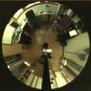
\includegraphics[width=0.15\textwidth]{cold/Freiburg_1PO(1)}
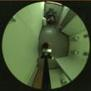
\includegraphics[width=0.15\textwidth]{cold/Freiburg_TL(1)}
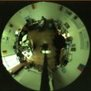
\includegraphics[width=0.15\textwidth]{cold/Ljubljana_LAB(1)}
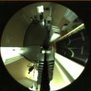
\includegraphics[width=0.15\textwidth]{cold/Ljubljana_PA(1)}
\end{center}
\caption{Sample data from the COLD database. Images were acquired from three diferent indoor laboratory enviroments located in diferent European cities: Saarbrücken, Freiburg and Ljubjlana.}
\end{figure}


\end{frame}

%%%%%%%%%%%%%%%%%%%%%%%%%%%%%%%%%%%%%%%%%%%%%%%%
%%%%%%%%%%%%%%%%%%%%%%%%%%%%%%%%%%%%%%%%%%%%%%%%
\section{Work Plan}
\begin{frame}{Work Plan}
\begin{figure}
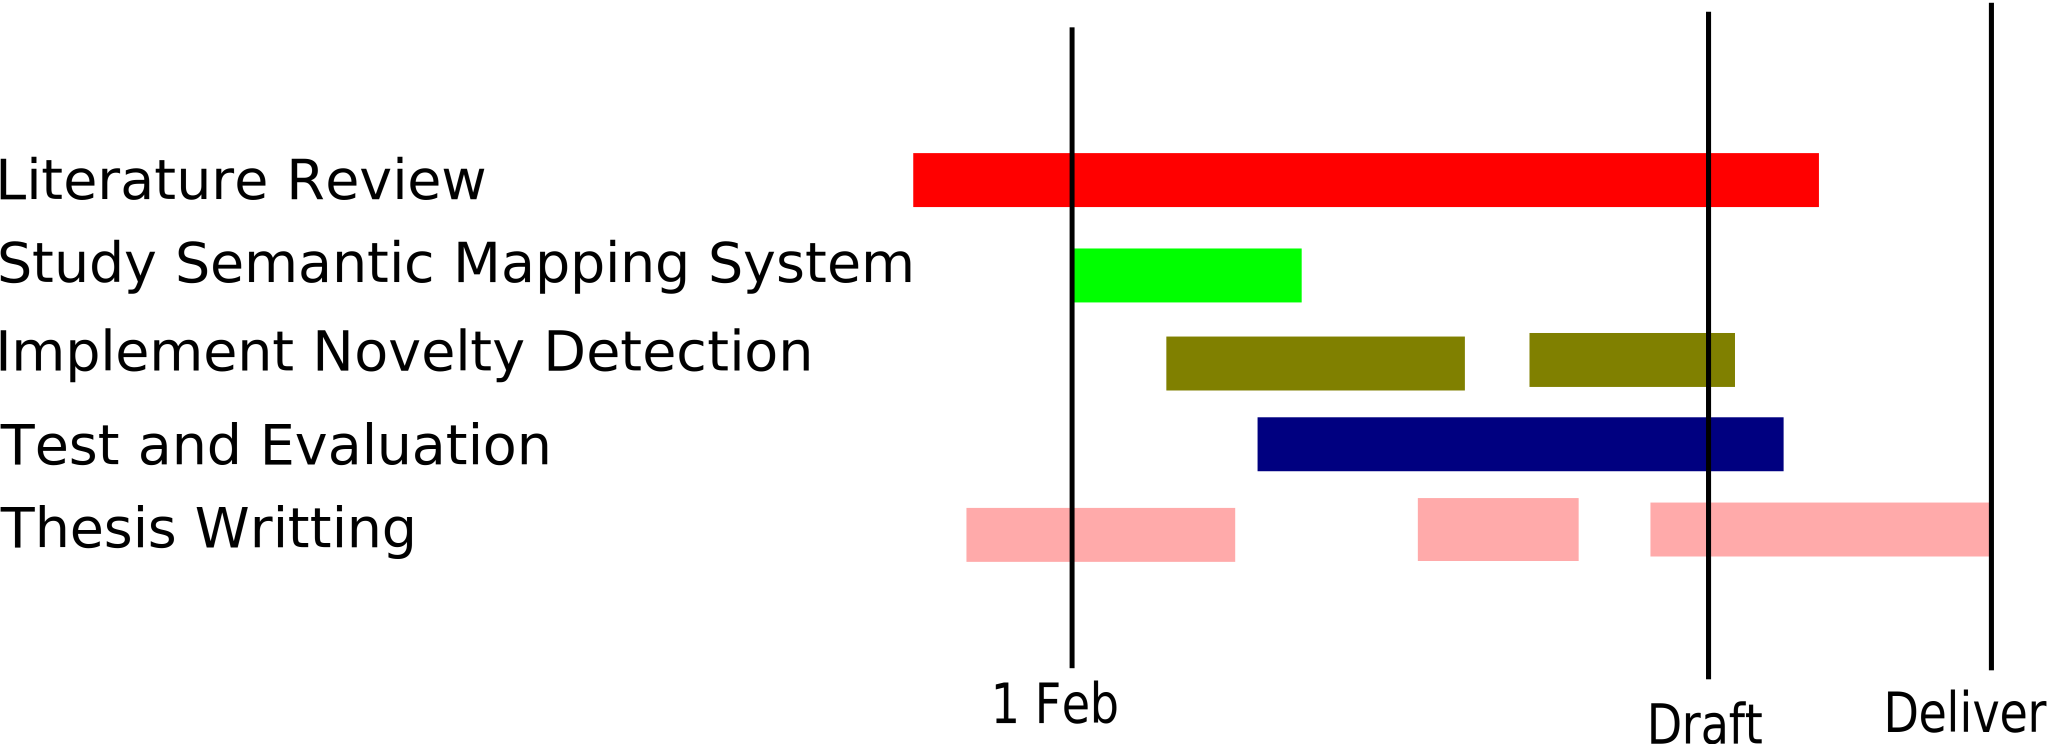
\includegraphics[width=\textwidth]{gantt.pdf}
\end{figure}

%    \begin{itemize}
%        \item Literature Review (3 weeks)
%        \item Study of the property-base semantic mapping system (2 weeks)
%        \item Implementing novelty detection algorithms (6 weeks)
%        \item Testing and evaluating methods (5 weeks)
%        \item Thesis writing (4 weeks)
%    \end{itemize}
\end{frame}


\appendix

\begin{frame}[allowframebreaks]{Bibliography}
\bibliographystyle{alpha}
\bibliography{myrefs}
\end{frame}

%\begin{frame}{Bibliography}
%Please consult the technical report.
%\end{frame}

\begin{frame}
    \titlepage
    Supervisors:
    \begin{itemize}
    \item Luis Paulo Reis
    \item Andrzej Pronobis
    \end{itemize}
\end{frame}


\end{document}
